%%%%%%%%%%%%%%%%%%%%%%%%%%%%%%%%%%%%%%%%%%%%%%%%%%%%%%%%%%%%%%%%%%%%%%%%%%%%%%%%
%2345678901234567890123456789012345678901234567890123456789012345678901234567890
%        1         2         3         4         5         6         7         8

\documentclass[letterpaper, 10 pt, conference]{ieeeconf}  % Comment this line out if you need a4paper

%\documentclass[a4paper, 10pt, conference]{ieeeconf}      % Use this line for a4 paper

\IEEEoverridecommandlockouts                              % This command is only needed if 
                                                          % you want to use the \thanks command

\overrideIEEEmargins                                      % Needed to meet printer requirements.

%In case you encounter the following error:
%Error 1010 The PDF file may be corrupt (unable to open PDF file) OR
%Error 1000 An error occurred while parsing a contents stream. Unable to analyze the PDF file.
%This is a known problem with pdfLaTeX conversion filter. The file cannot be opened with acrobat reader
%Please use one of the alternatives below to circumvent this error by uncommenting one or the other
%\pdfobjcompresslevel=0
\pdfminorversion=4

% See the \addtolength command later in the file to balance the column lengths
% on the last page of the document

% The following packages can be found on http:\\www.ctan.org
%\usepackage{graphics} % for pdf, bitmapped graphics files
%\usepackage{epsfig} % for postscript graphics files
%\usepackage{mathptmx} % assumes new font selection scheme installed
%\usepackage{times} % assumes new font selection scheme installed
%\usepackage{amsmath} % assumes amsmath package installed
%\usepackage{amssymb}  % assumes amsmath package installed
\usepackage{graphicx} % DO NOT CHANGE THIS
\usepackage{tabularx}
\usepackage{rotating} % For sideways in tabularx
\usepackage{paralist} %for inparaenum
\usepackage{amsmath}
\usepackage{caption}
\captionsetup[figure]{name={Figure}, labelsep=period}
\usepackage{lipsum}  
\usepackage{subfigure}
\usepackage{multirow}


\usepackage[capitalise,nameinlink]{cleveref} %Cref

%\usepackage[numbers]{natbib} 

\captionsetup[table]{position=bottom}   %% or below
\newcommand\pic[2][1]{\includegraphics[width=#1\linewidth,trim=2cm 2cm 2cm 2cm,clip]{fig/toy_sample_images/#2}}
\usepackage{tikz}
\newcommand{\igwc}[5]{\begin{tikzpicture}
	\draw (0, 0) node[inner sep=0] {\includegraphics[width=#1\linewidth]{#2}};
	\draw (#4, #5) node[fill=white,inner sep=1pt]  {\textbf{#3}};
	\end{tikzpicture}}

\title{\LARGE \bf
General and Robust Loss Function for Uncertainty Estimation}

\author{Deebul Nair$^{1}$, Nandhini Mathivanan$^{2}$, Miguel A. Olivares-Mendez$^{1}$ and Nico Hochgeschwender$^{3}$   % <-this % stops a space
\thanks{$^{2}$ Institute for Artificial Intelligence and Autonomous Systems, Bonn‑Rhein‑Sieg University of Applied Sciences, Grantham-Allee 20, 53757 Sankt Augustin, Germany.
        {\tt\small \{nandhini.mathivanan@smail.inf.h-brs.de, teena.hassan@h-brs.de t}}%
\thanks{$^{1}$ Space Robotics Research Group (SpaceR), Interdisciplinary Centre for Security, Reliability and Trust (SnT), University of Luxembourg, Luxembourg. {\tt\small miguel.olivaresmendez@uni.lu}}
\thanks{$^{3}$ University of Bremen, Germany. Department of Mathematics and Computer Science {\tt\small nico.hochgeschwender@uni-bremen.de}}%
}


\begin{document}



\maketitle
\thispagestyle{empty}
\pagestyle{empty}


%%%%%%%%%%%%%%%%%%%%%%%%%%%%%%%%%%%%%%%%%%%%%%%%%%%%%%%%%%%%%%%%%%%%%%%%%%%%%%%%
\begin{abstract}

%We present a generalization of negative log likelihood based uncertainty estimation.
%Our loss function generalizes algorithms built around negative log likelihood loss minimization by introducing a new robustness parameter, which improves performance on basic robotics tasks that involve noisy datasets.
%Interpreting our loss as the negative log likelihood of the generalized normal distribution results we get a general loss function that includes normal, Laplace and Cauchy functions as special cases.
%The use of robustness parameter enables the training of the DNN's in which the shape of the loss automatically adapts itself during training, thus improving performance on robotics tasks such as keypoint estimation and monocular depth estimation, even if  the training dataset contain noise and outliers.

%CGI format
The negative log likelihood loss function based uncertainty estimation often struggles with outliers in datasets, hindering the performance of deep neural networks (DNNs) in robotics applications. 
To address this limitation, we present a generalization of negative log likelihood based uncertainty estimation.
Our loss function generalizes algorithms built around negative log likelihood loss minimization by introducing a new robustness parameter, which improves performance on basic robotics tasks that involve datasets with outliers.
By generalizing the negative log likelihood loss, our approach extends its applicability to a wider range of distributions, including the normal, Laplace, and Cauchy distributions. This flexibility allows the DNN to dynamically adapt its learning process based on the percentage of outliers present in the dataset.
Our experiments show that the proposed loss function is significantly more resistant to outliers than existing uncertainty estimation methods, thus improving performance on robotics tasks such as keypoint estimation and antipodal grasping.
\end{abstract}


%%%%%%%%%%%%%%%%%%%%%%%%%%%%%%%%%%%%%%%%%%%%%%%%%%%%%%%%%%%%%%%%%%%%%%%%%%%%%%%%
\section{INTRODUCTION}
%Robustness
Robustness to outliers in data is an important factor when choosing a loss function for training deep neural networks(DNN). This is especially true in robotics tasks, where datasets often contain noisy labels and outliers.
This requirement also applies to uncertainty estimation methods, which are essential for deploying DNN in safety-critical robotics tasks \cite{borg_safely_2019, schwalbe_survey_2020}.
Researchers have developed various robust uncertainty estimation methods that can estimate correct uncertainty in the presence of outliers ~\cite{nair_laplace_2O22, barron2019general} .
Currently, roboticists spend considerable time either cleaning datasets or experimenting with different robust loss functions. 
%With different loss functions they compare both the estimated uncertainty and along-with minimum error. 
In this work, we aim to answer the following research question: \textit{When training a regression model on a dataset containing a certain percentage of outliers, how can the model accurately estimate the uncertainty of model's predictions by selecting the appropriate robust loss function?}

Uncertainty estimation in DNN is typically categorized into three main approaches: 
\begin{inparaenum}
	\item Bayesian methods \cite{kendall_what_2017, dusenberry2020analyzing}; \item Sampling based methods \cite{gal_dropout_2016, lakshminarayanan_simple_2016} and 
	\item Single model methods \cite{nix1994estimating} \cite{amini_deep_2019, sensoy_evidential_2018, nair_laplace_2O22}.
\end{inparaenum}
 While Bayesian and sampling-based methods often deliver state-of-the-art performance \cite{dusenberry2020efficient, wen2020batchensemble}, they come with significant computational overhead. Bayesian methods require doubling the model size and inference time \cite{blundell2015weight} , while sampling methods increase inference time substantially \cite{gal_dropout_2016, lakshminarayanan_simple_2016} . These drawbacks make them impractical for robotics applications that demand lean models and fast inference times. Single-model uncertainty estimation, on the other hand, can assess uncertainty with a single pass through the model and only a minimal increase in model size \cite{nix1994estimating, malinin_regression_2020, sensoy_evidential_2018} . Given its suitability for robotics systems, we focus on single-model uncertainty estimation in this work.

Negative likelihood-based loss functions offer a simple approach to uncertainty estimation in DNN. These methods model the output of the DNN as a statistical distribution, often the normal distribution. The loss function is then calculated as the negative log-likelihood (NLL) of the probability density function (PDF) of the chosen distribution. Studies have shown that using fat-tailed distributions like the Laplace distribution can make the model more robust to outliers in the data \cite{nair_laplace_2O22}. However, selecting the most appropriate distribution for a specific dataset still remains a manual process.

\begin{figure}
	\centering
	\begin{tabular}{cccc}
		\begin{sideways}
			\raggedright
            \scriptsize
			No Outliers 
		\end{sideways}
		&\pic[0.25]	{gaussian_4_layers_100_neuronsGaussian_0_0}
		&\pic[0.25]{ensemble_4_layers_100_neuronsEnsemble_0_0}
		&\pic[0.25]	{gaussian_4_layers_100_neuronsGeneralized_0_0}
		\\
		
		%(a) Gaussian &(b) Evidential \\
		%	\cite{nix1994estimating} & \cite{amini_deep_2019} \\
		%\pic[0.50]{ensemble_4_layers_100_neuronsEnsemble_0_100}
		\begin{sideways}
            \raggedleft
            \scriptsize
			10\%  Outliers 
		\end{sideways}
		&\pic[0.25]{gaussian_4_layers_100_neuronsGaussian_0_100}
		&\pic[0.25]{ensemble_4_layers_100_neuronsEnsemble_0_100}
		&\pic[0.25]{gaussian_4_layers_100_neuronsGeneralized_0_100}
		\\
		&(a) Gaussian &(b) Ensemble &(c) Generalized \\
		%	\cite{lakshminarayanan_simple_2016} &  \\ 
		
	\end{tabular}	
	
	%\vspace*{-3mm}
	\caption{Illustrative comparison of uncertainty estimation on 1D regression data with outliers. Row 1 shows data with no outliers while row 2 data contains 10\% outliers. The blue dots are clean data while red dots are outlier. The shaded blue region is the estimated uncertainty. Both Gaussian and Ensemble methods are more sensitive to outliers, the blue region are more distorted by the outlier data points, while for generalized the blue region has distorted less indicateing less impact of outliers.}
	\label{fig:toy-introduction}
\end{figure}


In this paper, we present a general uncertainty estimation loss function that is a super-set of common robust uncertainty estimation loss functions.
Our loss function is the negative log likelihood of the generalized normal distribution \cite{nadarajah2005generalized} . 
%The generalized normal distribution is parameterized by 2 parameter alpha and beta. 
%In our work we interpret the beta parameter as the robustness parameter. 
Using the negative log-likelihood of the generalized normal distribution as our loss function, we demonstrate that by minimizing the loss, any gradient-based optimization can automatically adjust the robustness of the loss without needing manual intervention.
This flexible form of our loss function is especially useful for models that produce high dimensional outputs, like those used for depth estimation and keypoint estimation. The loss function can assign a unique robustness value to each output dimension, allowing the model to adjust the robustness of its loss for each dimension individually. This robustness to outliers of our proposed loss function is demonstrated using a 1D regression dataset containing both heteroskedastic noise and outliers in \Cref{fig:toy-introduction}. Uncertainty predicted by Gaussian and Ensemble methods are heavily affected by outliers, while uncertainty predicted by our proposed method degrades the least while maintaining same accuracy.

This paper investigates the use of the generalized normal distribution \cite{nadarajah2005generalized} for maximum likelihood-based uncertainty estimation. Our work makes the following contributions:
\begin{compactenum}
	\item We propose a new loss function that adapts between multiple robust loss functions, based on the outliers in the data and thus improves the robustness of maximum likelihood-based uncertainty estimation methods;\par
	%	\item We use a proper scoring rule (Interval Score) as a metric to compare estimated uncertainties;\par
	\item We evaluate the estimated uncertainty on different regression benchmarks and also on a complex vision regression tasks of keypoint estimation; and\par
	\item We demonstrate and evaluate the use of estimated uncertainty by conducting a robotic experiment for grasp selection for antipodal grasp.\par
\end{compactenum}

\section{Robust Uncertainty estimation}
In a regression learning problem, we work with a training dataset $D$ that consists of pairs $(x, y)$ drawn from a joint distribution $D(X, Y)$. Each pair contains an input $x$ from the input set $X$ and a corresponding label $y$ from the label set $Y$.
We use a neural network $f(\theta)$, where $\theta$ represents the network's parameters. Our goal is to train these parameters by minimizing an empirical loss function $l$. This can be expressed as:
\begin{equation*}
\hat{\theta} = \underset{\theta}{\text{min}} R(\theta)  ;\quad  R(\theta) = \underset{<x,y> \in D}{E} [\ell (x,y,\theta)]
\end{equation*}
, where $R(\theta)$ is the expected loss over the dataset $D$.
In a standard regression scenario (without considering robustness or outliers), we can use the sum of squared residuals as our loss function:
\begin{equation*} 
\ell(x,y, \theta) = \frac{1}{2}(y - f_\theta(x))^2
 \end{equation*}   
 The square of residuals is a reformulation of the negative log likelihood of a normal distribution. This approach provides a point estimate, essentially estimating the mean ($\mu$) of a normal probability distribution. However, it's limited in its ability to provide uncertainty estimation. A straightforward enhancement to the basic regression model is to estimate the complete conditional probability distribution. This can be achieved by predicting both the mean ($\mu$) and the variance ($\sigma^{2}$) of the distribution, assuming it follows a Gaussian (normal) distribution. This approach, as described by \cite{nix1994estimating}, provides more information about the uncertainty of predictions.

Although the NLL of a normal distribution allows us to estimate both the value and the uncertainty in the prediction, it suffers from a lack of robustness. When the training data contains even a small number of outliers, it can lead to significant shifts in both the predicted values and their associated uncertainties.
This sensitivity to outliers means that these loss functions have a low tolerance for outlier data points. In statistical terms, these loss functions have a high breakaway point \cite{huber2004robust}.

For enhancing the robustness of NLL-based uncertainty estimation against outliers, various loss functions have been proposed utilizing fat-tailed distributions \cite{nair_laplace_2O22}. While these approaches have demonstrated effectiveness in mitigating the impact of outliers, the selection of the appropriate distribution hyperparameter often remains a manual process, relying on empirical experimentation.

In this work, we introduce a novel loss function that adaptively selects the suitable distribution based on the presence of outliers within the dataset. Our proposed loss function is grounded in the generalized normal distribution, a versatile distribution capable of representing different data distirbutions, including normal, Laplace, and Cauchy distributions. This flexibility enables our loss function to effectively model data with varying levels of tail behavior.



\begin{figure}[t]
	\centering
	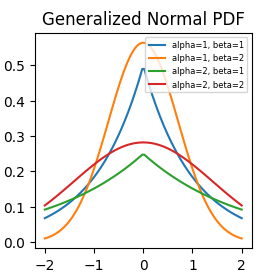
\includegraphics[width=0.45\linewidth]{fig/pdf.png}
 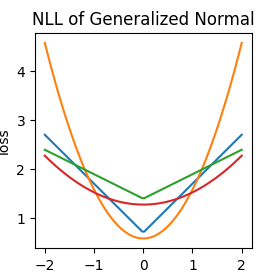
\includegraphics[width=0.45\linewidth]{fig/nll.png}
	%\vspace*{-10mm}
	\caption{Probability density function (PDF) (left) and negative log likelihood (NLL) (right) of Generalized normal distribution}
	\label{fig:nllgeneral}
\end{figure}

\subsection{Generalized Normal Loss Function}
The probability density function (PDF) of the generalized normal distribution is given by:
\begin{equation} 
p(r; \alpha, \beta) = \frac{\beta}{2\alpha\Gamma(1/\beta)} \exp \left[ -\left( \frac{|r|}{\alpha} \right)^{\beta} \right]
 \end{equation}   
where: $r$ is the random variable. $\alpha$ is the scale parameter ,controlling the spread of the distribution
and $\beta$  is the shape parameter, controlling the tail behavior of the distribution.
The parameters $\alpha$ and $\beta$ both are positive real numbers.
The NLL of the distribution is the loss function used for training. For the generalized normal distribution, the NLL can be derived from the PDF as follows: 
\begin{equation}
    NLL(\alpha, \beta; r) = -\sum_{i=1}^{N} \log f(r_i; \alpha, \beta)
\end{equation}
where: $N$ is the number of data points $r_i$ is the i-th error or residual.  \Cref{fig:nllgeneral}  plots both the PDF and the NLL for different values of $\alpha$ and $\beta$. Substituting the PDF into the NLL equation, we get:

\begin{equation}
   NLL(\alpha, \beta; r)  = \underbrace{ \left(\frac{\left|{r}\right|}{\alpha}\right)^{\beta}}_\textrm{term 1} - \underbrace{\log{\beta}}_\textrm{term 2} + \underbrace{\log{\left( 2\alpha \Gamma\left(\frac{1}{\beta}\right)\right) }}_\textrm{term 3}
\end{equation}

The loss function consist of 3 components : 
\begin{inparaenum}
    \item 
 term 1: This term measures the magnitude of the residual (error) between a predicted value and an actual value. The parameters $\alpha$ and $\beta$ control the shape and scale of this term.
     \item term 2 : These terms are regularization terms that help prevent over-fitting. They penalize large values of $\alpha$ and small values of $\beta$, which can lead to unstable models.
    \item term 3: This term involves the gamma function and it ensures that the loss function is well-defined for all values of $\alpha$ and $\beta$.
\end{inparaenum}
The proposed loss function has many properties that makes it suitable for gradient based optimization. 
\subsubsection{Differentiability} 
The loss function is differentiable almost everywhere. To show this, we can compute its partial derivatives with respect to $x$, $\alpha$, and $\beta$. Partial derivative with respect to r, for $r \neq 0 $ : 
    \begin{equation*}
    \frac{\partial L}{\partial r} = \beta \frac{|r|^{\beta-1}}{\alpha^{\beta}} \cdot \operatorname{sgn}(r)
\end{equation*}
for $r=0$:
\begin{equation*}
    \frac{\partial L}{\partial r} = 0
\end{equation*} . the partial derivative with respect to $\alpha$ 
\begin{equation*}
    \frac{\partial L}{\partial \alpha} = -\beta \frac{|r|^{\beta}}{\alpha^{\beta+1}} + \frac{2}{\alpha}
\end{equation*} and
the partial derivative with respect to $\beta$ 
\begin{equation*}
    \frac{\partial L}{\partial \beta} = \frac{|r|^{\beta}}{\alpha^{\beta}} \log \left( \frac{|r|}{\alpha} \right) - \frac{1}{\beta} + \frac{\Gamma'(1/\beta)}{\Gamma(1/\beta)}
\end{equation*}
From these expressions, we can see that the partial derivatives are continuous and defined for all $r$, $\alpha$, and $\beta$ except for r = 0. Therefore, the loss function is differentiable almost everywhere. This ensures that the gradient can be computed at most points, allowing the optimization algorithm to make progress.

\subsubsection{Unimodality} 
While the loss function is not strictly convex, it is generally unimodal. This means that there is a single global minimum. To show this, we can analyze the second-order partial derivatives:
Second-order partial derivative with respect to $r$:
\begin{equation*}
    \frac{\partial^2 L}{\partial r^2} = \beta (\beta-1) \frac{|r|^{\beta-2}}{\alpha^{\beta}}
\end{equation*}
From this expression we can see that the loss function is unimodal and thus has a single global minimum, making it easier for the optimization algorithm to converge to the optimal solution.

\subsubsection{Boundedness}
The loss function is bounded from below. The term $\log \Gamma{1/\beta}$ is bounded from below, and the remaining terms are non-negative. Therefore, the loss function cannot be arbitrarily negative.

Finally, the parameters $\alpha$ and $\beta$ can be interpreted as scale and shape parameters, respectively, providing insights into the behavior of the loss function.

\subsection{Different Uncertainty Estimation Loss Functions}
The generalized normal loss function consist of different NLL loss functions based on the $\beta$ parameter.
\subsubsection{Normal loss function}: When $\beta = 2$
\begin{equation*}
    NLL(\alpha, \beta=2; r) = \frac{r^2}{2\alpha^2} + 2\log{(\alpha)}
\end{equation*}
\subsubsection{Laplace loss function}: When $\beta = 1$
\begin{equation*}
     NLL(\alpha, \beta=1; r)  = \frac{|r|}{\alpha} + 2\log{(\alpha)}
\end{equation*}

\subsubsection{Cauchy loss function}: When $ {\beta \to \infty} $
\begin{equation*}
   NLL(\alpha, \beta \to \infty ; r) = \log \left( 1 + \frac{r^2}{\alpha^2} \right)
\end{equation*}

The generalized normal loss function provides a flexible framework for modeling different types of errors and can be adapted to specific needs by adjusting the parameters $\alpha$ and $\beta$.

\section{Related Work}
\label{sec:relatedwork}
\subsubsection*{{\textbf{Uncertainty Estimation}}}
In \cite{nix1994estimating} a novel approach was introduced for uncertainty estimation for neural networks by modeling outputs as Gaussian distributions and employing a negative log likelihood of the distribution as the loss function. This  method demonstrated the neural network's ability to learn both predictions and uncertainty. In \cite{blundell2015weight}, DNN uncertainty estimation was achieved by representing network weights with distributions. \cite{gal_dropout_2016} proposed a sampling based techniques using dropouts and multiple forward passes and capture the differences in the different passes as uncertainty.
Ensemble methods, as exemplified by \cite{lakshminarayanan_simple_2016, dusenberry2020efficient} and \cite{wen2020batchensemble} currently dominate state-of-the-art uncertainty estimation. These methods leverage multiple models within a single framework to provide robust uncertainty estimates. Despite their effectiveness, ensemble methods generally necessitate multiple forward passes, limiting their applicability in real-time or resource-constrained scenarios.
\subsubsection*{{\textbf{Single Inference Uncertainty Estimation}}}
Several methods can estimate uncertainty using a single inference. These include:
\begin{inparaenum}
    \item Replacing the loss function with NLL of statistical distribution \cite{malinin_regression_2020, sensoy_evidential_2018, amini_deep_2019, nair_laplace_2O22},
    \item Computing the closed-form posterior for the output layer \cite{Riquelme2018Deep, SnoekRSKSSPPA15},
    \item Changing the output layer \cite{calandra2016manifold, tagasovska2019single}, 
    \item Using spectral normalization \cite{LiuLPTBL20} and
    \item Applying a two-sided gradient penalty  \cite{van2020uncertainty}
\end{inparaenum}
\subsubsection*{{\textbf{Robust Uncertainty Estimation}}}
Robust training in the presence of outliers is a classic statistical problem often addressed using M-estimators \cite{huber2004robust}. For DNN, \cite{barron2019general} proposed a generalized M-estimator loss function that uses the negative log of the density function to improve robustness during training. \cite{lathuiliere2018deepgum} introduced a Gaussian-uniform mixture model as a loss function that can continuously adapt to outliers in the data. In \cite{nair_laplace_2O22} studied the usage of Laplace NLL as loss function for improving robustness to outliers. 
In this work we work on a extension of this work which generalizes different fat tailed distribution based NLL loss function thus further improving robustness capability of DNN.

\section{EVALUATION}
In this section, we evaluate the performance of our proposed loss function. Our focus is on demonstrating its ability to improve robustness to outliers in the data. While these benchmarks do not aim to represent the state-of-the-art for any specific task, they effectively showcase the capabilities of our loss function in learning uncertainty with outlier-contaminated datasets. For comparison, we consider the following uncertainty estimation methods: \textbf{Gaussian}, as introduced in \cite{nix1994estimating}, \textbf{Ensemble}, corresponding to the deep learning ensemble approach proposed by \cite{lakshminarayanan_simple_2016}, \textbf{Evidential}, utilizing the Normal-inverse-Gamma distribution as suggested by \cite{amini_deep_2019},  \textbf{Laplace}, as described in \cite{nair_laplace_2O22} and \textbf{Generalized} method described in this paper.
%We evaluate these methods on a variety of tasks to demonstrate their performance in uncertainty prediction in the presence of outliers. These tasks include a 1D outlier regression dataset, real-world regression datasets, and a robotics keypoint estimation task. 
%These datasets were specifically chosen due to the presence of outliers, making them ideal for testing the robustness of our methods. 
%Additionally, we showcase a practical application of uncertainty estimation by conducting a robot grasping experiment using keypoints predicted by different uncertainty estimation methods. 
%This experiment highlights the real-world impact of accurate uncertainty quantification in robotic tasks. 
We formulate our experiments to answer the following questions:
\begin{enumerate}
    \item \textbf{RQ1}: How does DNN trained using Generalized NLL compare with other uncertainty estimation methods on different regression benchmarks ?
    \item \textbf{RQ2}: How much percentage of outliers can the different methods handle before their prediction and uncertainty deteriorates ?
    \item \textbf{RQ3}: How does the proposed loss function compare for a complex vision task of Key point estimation ?
    \item \textbf{RQ4}: How can the uncertainty predicted by the keypoint estimation DNN be used for improving grasping and how do they compare with each other ?
\end{enumerate}

\begin{table}[t]
\centering
\begin{tabular}{l|r|r|r|r|r}
 & Ensemble & Evidential & Gaussian & Laplace & Ours \\
 \hline
boston & 1.24 & 1.55 & 1.60 & 1.29 & \textbf{1.23} \\
concrete & 1.45 & 570.23 & 1.89 & 1.62 & \textbf{1.42} \\
energy & 0.70 & 51.54 & 0.88 & 0.84 & \textbf{0.65} \\
kin8nm & 1.25 & 882.00 & 1.69 & 1.43 & \textbf{1.19} \\
naval & \textbf{0.95} & 640.84 & 1.11 & 1.25 & 1.10 \\
power & 0.94 & 599.59 & 1.34 & 1.07 & \textbf{0.93} \\
protein & 3.01 & 397.89 & 4.13 & 3.48 & \textbf{2.91} \\
wine & 3.61 & 4.52 & 4.27 & 3.96 & \textbf{3.17} \\
yacht & 0.37 & 0.33 & 0.47 & 0.43 & \textbf{0.32} \\
 \hline

\end{tabular}
\caption{Interval Score for different uncertainty estimation methods trained on different UCI datasets. Our proposed Generalized NLL loss function consistently outperforms most of the  baselines. }
\label{tab:ISTable}
\end{table}

\begin{figure}[t]
	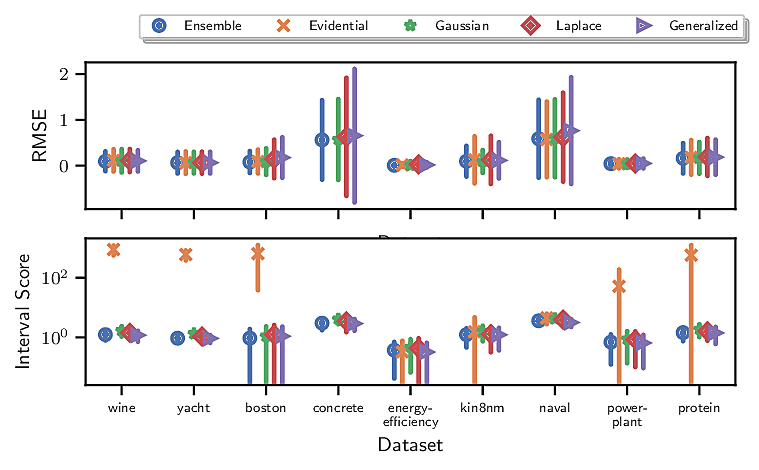
\includegraphics[width=\linewidth]{fig/RMSE_IS_Comb_point_uci.png}	
	\caption{\textbf{Benchmark Regression Tasks}: RMSE and Interval Score box plot for comparison. The RMSE for all the methods are comparable and lie in same region. Interval score which predicts the quality of uncertainty estimation we can see that some methods the score degrades even though their RMSE score is good.
		\label{fig:benchmarkRegression}
	}
\end{figure}


\begin{figure}[b]
	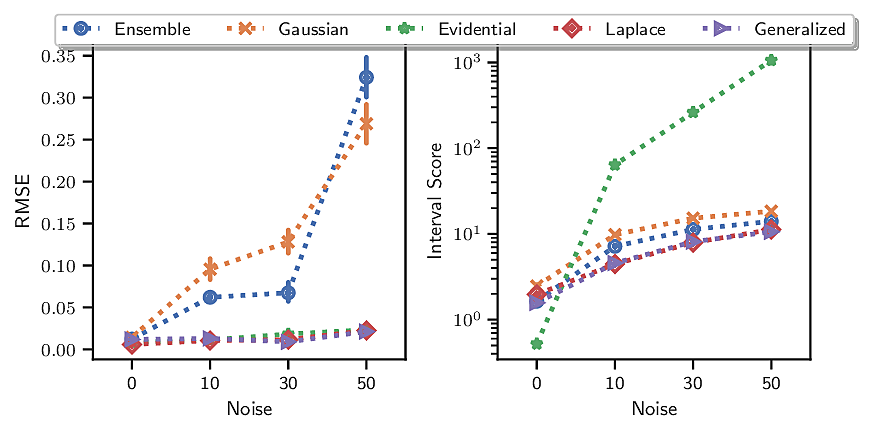
\includegraphics[width=\linewidth]{fig/noise_RMSE_IS_point_plot.png}	
	\caption{\textbf{Breakaway Point estimation}: The change in RMSE and Interval Score with respect to outlier percentage in the data for 1D regression dataset.  
		%In the first row with clean data all the methods estimate the underlying data and the uncertainty accurately. With increasing outliers the uncertainty estimates get mis alligned. You can observe the Laplace loss function is able to correctly estimate the underlying data even with 50\% outliers
		\label{fig:breakawayExperiment}
	}
\end{figure}

\subsection{Benchmark Regression Tasks}
To answer RQ1, we benchmark our uncertainty estimation method on real-world regression datasets. 
To evaluate a DNN's ability to estimate uncertainty accurately, we need metrics that separate the quality of uncertainty from the quality of predictions. Scoring rules are a group of metrics that assess uncertainty quality by assigning a numerical score based on both predictions and uncertainty \cite{gneiting2007strictly}.
We use the Interval Score scoring rule, which compares prediction intervals.
The Interval Score rewards narrow predictions and penalizes predictions outside the interval. We set $\alpha$ of Interval score to 95\% for our experiments. 
%Based on the neural network's predicted mean and variance, we calculate the 95\% quantile prediction interval (l, u). This interval is then used to compute the Interval Score. 
Because the Interval Score compares the 95\% quantile prediction interval, it's comparable across different distributions.
We conducted 20 experiments with random training and testing data splits. We used a fully connected neural network with Adam optimization and a learning rate of $5e^{-3}$. Our results show that our proposed method performs the best as compared to other methods in terms of Interval Score as show in \Cref{tab:ISTable}.



\begin{figure*}[htbp!]
	\centering
	\igwc{0.31}{fig/cornell_data.png}{\textbf{A}}{-2.5}{1.7}
	\igwc{0.32}{fig/keypoint-RMSE.png}{\textbf{B}}{-1.9}{1.7}
	\igwc{0.31}{fig/keypoint-IS.png}{\textbf{C}}{-2.05}{1.7}
	\caption{\textbf{Keypoint Estimation} Trained on Cornell Grasp Dataset. \textbf{(A)} Example images from dataset.\textbf{ (B)} RMSE comparison plot \textbf{(C)} Interval score plot. Genralized NLL trained model have the lowest RMSE and Interval scores as compared to other uncertainty estimation methods.}
	\label{fig:keypointrsults}
\end{figure*}

\subsection{Empirical Breakaway Point }
To answer RQ2 about the robustness of different loss functions to outliers, we conducted experiments using a 1D regression problem with increasing outliers in dataset. We employed a 4-layer neural network and systematically introduced outliers, ranging from 0\% to 50\% of the total data. The "breakaway point" was determined by observing the threshold at which a method's performance began to deteriorate significantly. This method provided insights into how well each loss function could withstand the presence of outlier data points and maintain accurate predictions and uncertainty. 
For each experiment, we recorded the RMSE and Interval Score to gauge both prediction accuracy and uncertainty estimation quality. 

Our findings as shown in \Cref{fig:breakawayExperiment} revealed that Gaussian and Ensemble methods exhibited similar levels of robustness, breaking down at approximately 10\% outlier contamination. However, Evidential learning, while demonstrating strong performance in uncertainty estimation, was less resilient to outliers in terms of prediction accuracy, breaking down at around 10\% as well.
We observe how both fat tailed loss function Laplace and Generalized was able to sustain performance even in the presence of 50\% outliers.  
These results underscore the importance of comprehensive evaluation in assessing the robustness of uncertainty estimation models. While a method might excel in one aspect, such as uncertainty estimation, it may be susceptible to outliers in another, such as prediction accuracy. Therefore, it is crucial to consider both factors when selecting a suitable method for a given application.

\begin{table}[b]
\centering
\begin{tabular}{ c|c|c }
Dataset & RMSE & Interval Score \\
 \hline
Gaussian & 0.0469 & 1.7960  \\
Laplace  & 0.0459 & 0.4348   \\
Ensemble  &  0.0477 & 0.9202  \\
Evidential  & 0.0729 & 1.1217  \\
Generalized (Ours) & \textbf{0.0411} & \textbf{0.4331}  \\
\hline
\end{tabular}
\caption{RMSE and Interval Score Result table for Cornell Grasp dataset}
\label{tab:Cornel}

\end{table}

\subsection{Keypoint Estimation}
Having established benchmark comparison results, we now demonstrate the scalability of our generalized NLL learning approach by applying it to the complex, high-dimensional task of keypoint estimation. 
Keypoint estimation is a computer vision task that involves identifying and locating specific points of interest within an image. It's essentially a regression problem, where the goal is to predict the continuous x and y coordinates of each keypoint within the image. Its a challenging task due to the high-dimensional nature of the target output, with predictions required at every pixel. 

\textit{Cornell grasp dataset and Data Augmentation}
We train our model using the Cornell grasp dataset \cite{lenz2015deep}. The Cornell Grasp Dataset is a collection of real-world images and corresponding annotations for robotic grasping tasks. It contains a diverse range of objects, including everyday items like cups, bottles, tools, and toys. Each image is paired with annotations that specify the most suitable pinch grasp points. The Dataset contains around 1K RGB-D images of 240 different objects. \Cref{fig:keypointrsults} A shows a sample of training images from the dataset. Each image has dimension of 640 × 480px and is annotated with multiple potential grasp points, typically ranging from 1 to 10 per image. 
To address the limited size of the dataset, we implemented data augmentation techniques to increase its diversity during training.
Data augmentation methods of random rotations between 0 and 360 degrees were applied, along with random translations in the x and y directions of up to 50 pixels. 
%These augmentations helped improve the model's generalization capabilities by exposing it to a wider range of variations in the data.

\begin{figure*}[t]
    \centering
    \subfigure[]
    {
        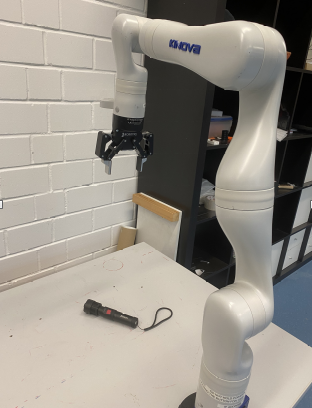
\includegraphics[width=0.2\linewidth]{fig/kinova.png}
    }
    \qquad
     \centering
     \subfigure[]
    {
    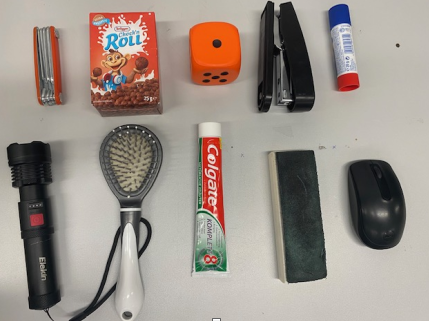
\includegraphics[width=0.3\linewidth]{fig/objects.png}
    }
    \qquad
    \subfigure[]
    {
    \begin{tabular}[b]{l|c}
        Method & Success Rate ($\uparrow$)\\
        \hline
        Gaussian & 36.2 $\%$\\
        Laplace & 58.3 $\%$\\
        Cauchy & 33.1 $\%$\\
        Evidential & 31.9 $\%$\\
        \textbf{Generalized (ours)} & \textbf{61.5} $\%$\\
        \hline
    \end{tabular}
    \captionlistentry[table]{A table beside a figure}
    \label{tableGrasp}
    }
    %\captionsetup{labelformat=andtable}
    \caption{Robot grasp benchmark: (a) Experimental setup consisting of a kinova arm with intel realsense camera on its tooltip with one object placed in front of robot for grasping. (b) Novel 10 objects selected for the experiments (c) Table with results of the benchmark }
\end{figure*}
\textit{Architecture:} 
We utilized a ResNet18 architecture \cite{he2016deep} as our architecture. The neural network's output is an 8x2 matrix, representing 8 keypoints with x and y coordinates. For Gaussian and Laplace networks, the output expands to 8x4, adding two dimensions for the scale parameter. Evidential networks have an 8x8 output, with three additional outputs for each keypoint. Generalized NLL networks output 8x6.  The hyperparameters used are Adam optimization, learning rate of 1e-3, batch size of 32, and 200 training epochs. 
\textit{Training Schedule:}
The network was trained end-to-end using Adam as the optimizer with a learning rate of 1e-3, weight decay of 0.001, a momentum factor of 0.9, and momentum enabled. We used a batch size of 32 and trained the nodels with each loss function for 200 epochs.

\textit{Quantitative Results:}
\Cref{tab:Cornel} presents the results on the Cornell grasp dataset. The detailed box plot of the RMSE and Interval scores are plotted in \Cref{fig:keypointrsults} B and C respectively. Our loss function achieves state-of-the-art accuracy compared to other NLL loss functions. Notably, our Generalized NLL method also outperforms other NLL methods in terms of Interval Score. 
%The box plot of the RMSE and Interval scores are plotted in \Cref{fig:keypointrsults} B and C respectively. 
This shows that our Generalized NLL loss function is able to adjust the shape of the loss function based on the outliers present in the data and is able to adjust. 
%This also demonstrates that Generalized NLL can be applied to high dimensional dataset task and performs in a comparative manner. 


\subsection{Uncertainty Estimation Based Grasping}
In order to study RQ4, we conducted an experiment where the uncertainty can be used on a robotics task and we can benchmark the different lo function on robotics task. We deployed the keypoint estimation DNN models learned in the previous section on a robot arm for object grasping using antipodal grasp. We leverage the predicted uncertainties, into developing a robust grasp selection algorithm. This algorithm chooses the optimal keypoint for physical grasping by selecting a single best keypoint with least uncertainty from the 8 keypoints predicted by the model for each object.

In this experiment, we used a Kinova robot arm equipped with a Robotiq gripper end-effector for object grasping. Ten objects were selected from the Cornell Grasp dataset, as illustrated in Figure . An Intel Realsense camera is available on the robot's end-effector. The objects were arranged on a horizontal surface with a white background in a region with optimal reachability.
We use the grasp protocol as recommended in previous research by \cite{bekiroglu2019benchmarking}. Our experiment employs a top-down grasping approach for single objects on a table. Each object is positioned at a predetermined location and orientation relative to the robot. The keypoint estimation algorithm identifies potential grasping points, and the grasp selection algorithm chooses the most suitable keypoint. The grasp planner then converts this keypoint into 3D world coordinates and commands the robot arm to execute the grasp. This process is repeated N times for comprehensive evaluation.
As outlined in \cite{bekiroglu2019benchmarking}, the results can be evaluated using the metric $s/a$, where $s$ represents the count of successful grasps and $a$ equals $2 * N$, with $N$ being the number of grasp attempts per object. The factor of 2 accounts for the consideration of two different object orientations: vertical and horizontal. Grasp failures are identified when the gripper displaces the object, when the object slides or moves during grasping or lifting, or when the grasped item is dropped. This experimental setup is valuable for determining the optimal grasping pose using uncertainty estimation methods and can be evaluated based on the aforementioned criteria.

A final success rate, calculated as the normalized average across all trials and poses is reported in \Cref{tableGrasp} . 
We observe that the DNN trained with Generalized NLL performs the best with $61.5 \%$ success rate in grasping.

  
\section{DISCUSSION}

We introduced a generalized loss function that can adapt its shape to outliers in the dataset. This eliminates the need for researchers to manually select a suitable loss function, as the model automatically adjusts to find the appropriate loss function and corresponding distribution.
To evaluate the performance of our DNN model trained with this loss function, we tested it on a datasets with varying percentages of outliers. Our results demonstrated that the model trained with generalized NLL loss function is robust to outliers, with minimal impact on both performance and estimated uncertainty.
We also benchmarked our loss function on various regression benchmarks and found it to achieve state-of-the-art with respect to uncertainty estimation. Additionally, we applied it to the high-dimensional task of keypoint estimation. Furthermore, we demonstrated the practical utility of the predicted uncertainty in a robotics task: robot grasping.

While our work provides a proof of concept for using this loss function in DNN training, further research is needed to explore its runtime robustness. Adversarial testing and out-of-distribution detection are areas that warrant investigation. We hope that these efforts will contribute to the development of stable uncertainty estimation methods that are resilient to outliers.
\addtolength{\textheight}{-12cm}   % This command serves to balance the column lengths
                                  % on the last page of the document manually. It shortens
                                  % the textheight of the last page by a suitable amount.
                                  % This command does not take effect until the next page
                                  % so it should come on the page before the last. Make
                                  % sure that you do not shorten the textheight too much.


\section*{ACKNOWLEDGMENT}
Deebul Nair gratefully acknowledges the on-going support
of the Bonn-Aachen International Center for Information Technology and a PhD
scholarship from the Graduate Institute of the Bonn-Rhein-Sieg University. 
%Thiswork was supported by the European Union’s Horizon 2020 project SciRoc (grantagreement No. 780086), SESAME (grant agreement No. 101017258) and DLRCASSy project.

%%%%%%%%%%%%%%%%%%%%%%%%%%%%%%%%%%%%%%%%%%%%%%%%%%%%%%%%%%%%%%%%%%%%%%%%%%%%%%%%

\bibliographystyle{IEEEtran}
\bibliography{root}


\section*{SUPPLEMENTARY MATERIALS}
\subsubsection{Interval Score} uses the prediction interval, with lower and upper endpoints represented by predictive quantiles at level $\frac{\alpha}{2}$ and $1 - \frac{\alpha}{2}$. The Interval Score is defined as :
\begin{equation}
S_\alpha^{int} (l,u;y) = (u - l) +\frac{2}{\alpha}(l-y)\mathbf{1}\{y<l\} + \frac{2}{\alpha}(y-u)\mathbf{1}\{y>u\}
\end{equation}


\subsubsection{Robot grasping experiment individual experiment }

Experiment results of individual obejcts 
\begin{table}[htbp]
	\caption{Result table from grasping experiment}
	\centering
	\begin{tabular}{|l|c|c|c|c|c|c|c|c|c|c|}
		\hline
		
		 & \multicolumn{2}{c|}{\textbf{Generalized}} & \multicolumn{2}{c|}{\textbf{Gaussian}} & \multicolumn{2}{c|}{\textbf{Laplace}} & \multicolumn{2}{c|}{\textbf{Cauchy}} & \multicolumn{2}{c|}{\textbf{Evidential}} \\ \cline{2-11} 
		
		& P1 & P2 & P1 & P2 & P1 & P2 & P1 & P2 & P1 & P2 \\ \hline
		Torch & 9 & 5 & 6 & 2 & 8 & 5 & 5 & 0 & 4 & 0 \\ \hline
		Marker & 9 & 4 & 7 & 1 & 7 & 2 & 5 & 1 & 5 & 1 \\ \hline
		Mouse & 4 & 3 & 2 & 2 & 3 & 2 & 2 & 3 & 4 & 3 \\ \hline
		Brush & 5 & 4 & 4 & 3 & 6 & 4 & 3 & 1 & 3 & 0 \\ \hline
		Stapler & 6 & 7 & 1 & 4 & 3 & 5 & 1 & 3 & 1 & 2 \\ \hline
		Paste & 8 & 8 & 4 & 4 & 8 & 7 & 5 & 5 & 4 & 3 \\ \hline
		Cube & 6 & 6 & 5 & 5 & 6 & 6 & 5 & 5 & 5 & 5 \\ \hline
		Duster & 6 & 5 & 4 & 2 & 7 & 5 & 2 & 1 & 3 & 0 \\ \hline
		Box & 9 & 4 & 7 & 3 & 9 & 3 & 7 & 2 & 7 & 1 \\ \hline
		Allen & 10 & 5 & 4 & 2 & 9 & 2 & 8 & 2 & 8 & 3 \\ \hline
		
	\end{tabular}
	
\end{table}


\subsubsection*{LIMITATIONS}

The proposed loss function is not convex in general. 
To demonstrate non-convexity, consider the following scenario:
Fixed $\alpha$, Let $\alpha = 1$.
Varying $r$, Choose two points $r1 = 1$ and $r2 = -1$.
Convexity condition: A function f is convex if for all $r1$, $r2$ and $\lambda \in [0, 1]$:
\begin{equation*}
    f(\lambda x1 + (1-\lambda) x2) \leq \lambda f(x1) + (1-\lambda)L(x2)
\end{equation*}
Evaluating the loss function:
\begin{equation*}
L(r1) = 1 - log(\beta) + log(\Gamma(1/\beta))
\end{equation*}
\begin{equation*}
L(r2) = 1 - log(\beta) + log(\Gamma(1/\beta)) \\
\end{equation*}
\begin{equation*}
L(\lambda r1 + (1-\lambda)r2) = | \lambda - (1-\lambda)|^\beta - log(\beta) + log(\Gamma(1/\beta))
\end{equation*}
Checking the convexity condition:
For $\lambda$ = 0.5:
\begin{equation*}
   L(0.5r1 + 0.5r2) = 0 - log(\beta) + log(\Gamma(1/\beta)) 
\end{equation*}
\begin{multline*}
\lambda L(r1) + (1-\lambda)L(r2) \\ 
0.5(1 - log(\beta) + log(\Gamma(1/\beta))) \\ + 0.5(1 - log(\beta) + log(\Gamma(1/\beta))) = 1 - log(\beta) + log(\Gamma(1/\beta))
\end{multline*}
The convexity condition is not satisfied for all $\lambda \in [0, 1]$. Therefore, the loss function is not convex.
While the loss function is not globally convex, it might be locally convex under certain conditions. However, the general form presented here does not guarantee convexity. 
We overcome this limitation by adding a software ode by clamping the loss to the very small number as possible in the cpu. This ensures that the residual never becomes zero and thus 


\end{document}
